%!TEX root = ../../secondYearReport.tex

% 1.68 man.months for UPMC on T4.4 

Within T4.4, UPMC studied how to deal with interferences between tasks using
machine learning tools. Whole-Body Control methods offer the potential to
execute several simultaneous tasks on highly redundant robots, such as
humanoids. Unfortunately, task combinations often result in interferences or
incompatibilities which generate undesirable behaviors. Prioritization schemes
between tasks, such as strict and soft hierarchies, are typically used to manage
these interferences but generally require a deal of time consuming and arbitrary
tuning.

To circumvent theses issues, UPMC presented a novel framework for defining and
optimizing multiple tasks in order to resolve potential interferences prior to
task execution. In a first study \cite{lober-HUMANOIDS2014} the tasks are
parameterized with Dynamical Movement Primitives, whose parameters are optimized
based on a general compatibility principle, which is independent of the robot’s
topology, tasks or environment. Two test cases on a simulation of a humanoid
robot are used to demonstrate the successful optimization of initially
interfering tasks. A video summarizing the outcome of this work can be viewed
\href{http://pages.isir.upmc.fr/~padois/website/fichiers/videos/lober_Humanoids2014.mp4}{here}.

\begin{figure*}
\centering
\begin{subfigure}{.31\linewidth}
 \centering
 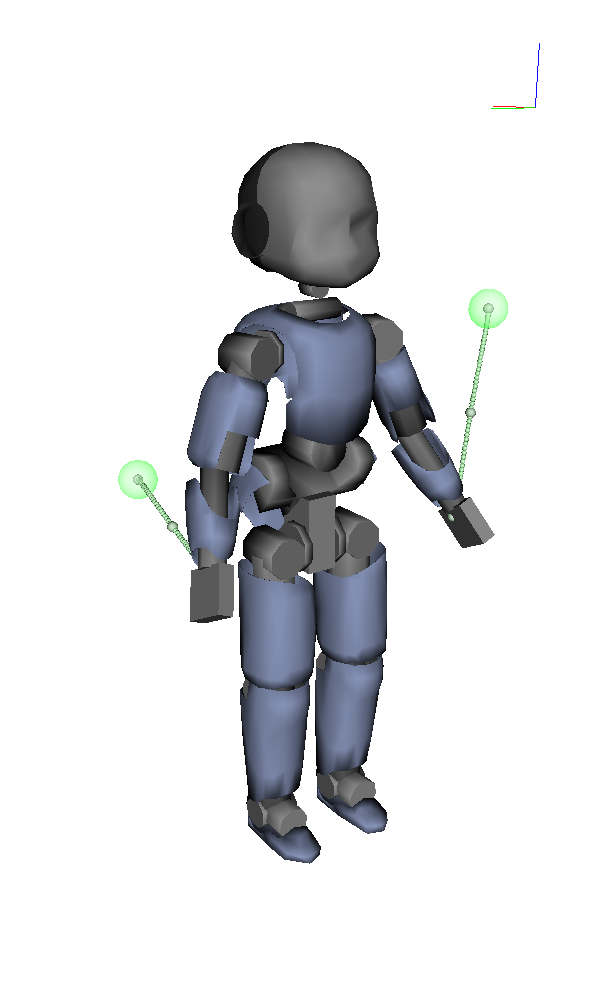
\includegraphics[trim = 0cm 4.5cm 0cm 5cm, clip, height=4 cm]{./sections/WP4/pics_UPMC/01_starting}
 \caption{Constrained Configuration}
 \label{fig:config}
\end{subfigure}
%
\begin{subfigure}{.31\linewidth}
 \centering
 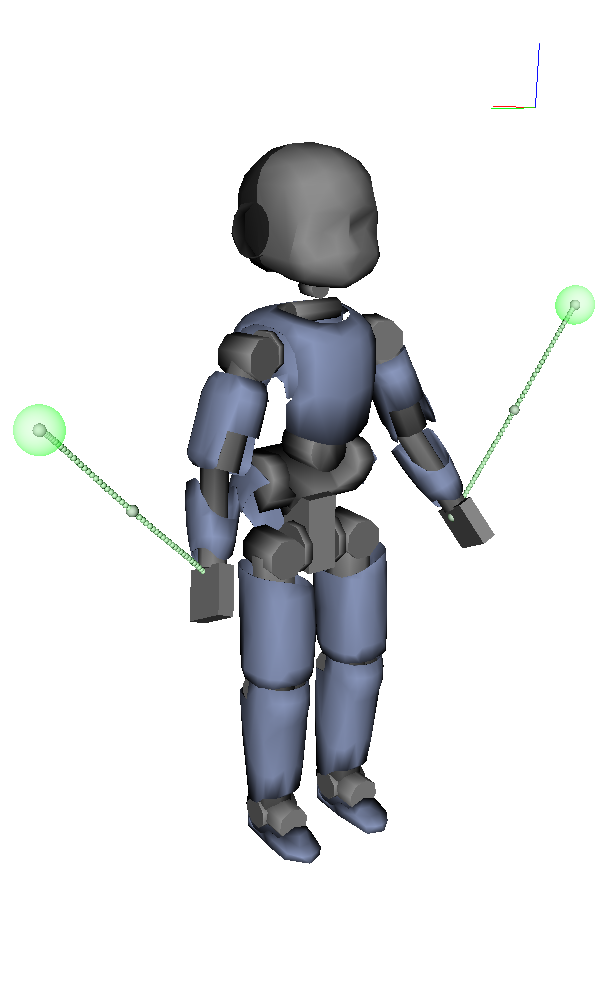
\includegraphics[trim = 0cm 4.5cm 0cm 5cm, clip, height=4 cm]{./sections/WP4/pics_UPMC/02_starting}
 \caption{Workspace Violation}
 \label{fig:work}
\end{subfigure}
%
\begin{subfigure}{.31\linewidth}
 \centering
 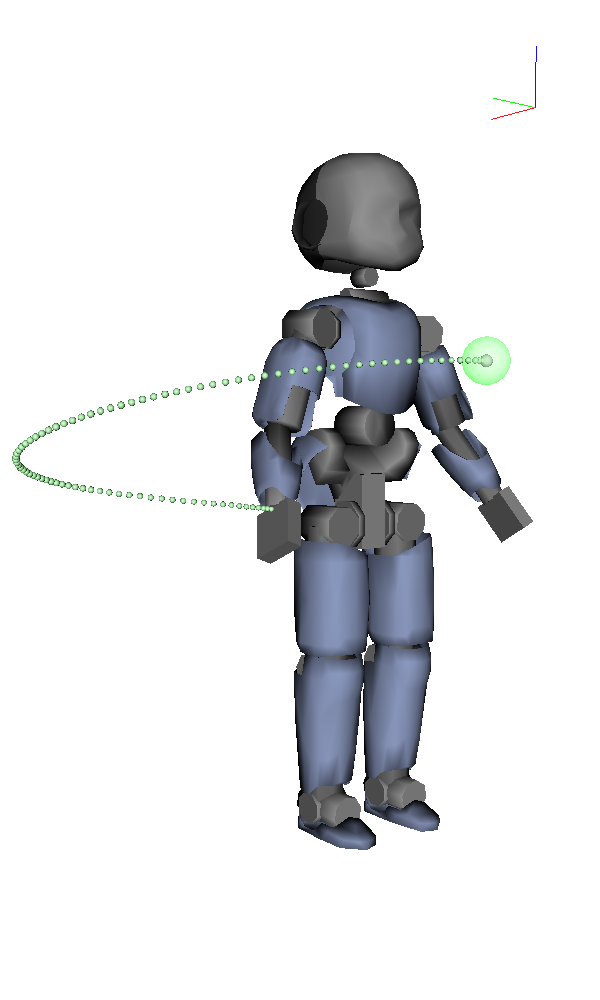
\includegraphics[trim = 0cm 5cm 0cm 5cm, clip, height=4 cm]{./sections/WP4/pics_UPMC/03_starting}
 \caption{Balance Perturbation}
 \label{fig:balance}
\end{subfigure}
%
\caption{Three common multi-task incompatibility scenarios. The desired hand
task trajectories are indicated by the green markers. Medium size spheres
represent waypoints, and large transparent spheres represent the final waypoints
or goals.}
\label{fig:3_scenarios_lober_2015}
\end{figure*}


In a second study \cite{lobersubmittedIROS2015}, UPMC studied how task
variability can be used to modulate task priorities during their execution, to
temporarily deviate certain tasks in the presence of incompatibilities. A method
for mapping from task variance to task priority was presented as well as an
approach for calculating task variance for generated trajectories. The method
successfully resolved three common task conflict scenarios online illustrated on
Fig.~\ref{fig:3_scenarios_lober_2015}.



% Refs to add to secondYearReport_WP4.bib




